\documentclass[11pt,a4paper]{article}
\usepackage[T1]{fontenc}
\usepackage[utf8]{inputenc}
\usepackage[main=american,finnish]{babel}
\usepackage{lmodern}
\usepackage{microtype}
\usepackage[margin=22mm,headheight=44pt,headsep=8mm,footskip=12mm]{geometry}
\usepackage{graphicx}
\usepackage[dvipsnames]{xcolor}
\usepackage{booktabs,tabularx,array,longtable}
\usepackage{enumitem}
\usepackage{amsmath,amssymb}
\usepackage{caption}
\usepackage{float}
\usepackage{fancyhdr}
\usepackage[most]{tcolorbox}
\usepackage[hidelinks]{hyperref}
\usepackage{url}

\definecolor{UTUBlue}{HTML}{005F86}
\definecolor{UTULight}{HTML}{EAF3F7}
\definecolor{UTUDark}{HTML}{263746}
\definecolor{SoftGray}{HTML}{F3F5F6}
\definecolor{WarnGold}{HTML}{F6E8B1}
\newcommand{\StudyTitle}{To Renounce Liberty? A Public-Goods Experiment on (Un)Democratic Reversal}
\newcommand{\StudyTitleFI}{Luopuako vapaudesta? Julkishyödykekoe (epä)demokraattisesta suunnanmuutoksesta}
\newcommand{\StudyPI}{Janne Tukiainen}
\newcommand{\StudyEmail}{\href{mailto:janne.tukiainen@utu.fi}{janne.tukiainen@utu.fi}}
\newcommand{\StudyPhone}{+358 50 308 3620}
\newcommand{\DocumentDate}{31 August 2026}
\newcommand{\DocumentVersion}{Version 2.0}
\newcommand{\checkbox}{$\square$}

\pagestyle{fancy}
\fancyhf{}
\fancyhead[L]{
\includegraphics[height=13mm]{utu_logo.pdf}}
\fancyhead[R]{\footnotesize\color{UTUDark}\StudyTitle}
\fancyfoot[L]{\footnotesize\color{UTUDark}\DocumentVersion\ -- \DocumentDate}
\fancyfoot[R]{\footnotesize\color{UTUDark}\thepage}
\renewcommand{\headrulewidth}{0.35pt}
\renewcommand{\footrulewidth}{0.25pt}
\setlength{\parindent}{0pt}
\setlength{\parskip}{0.55em}
\setlist{nosep,leftmargin=1.35em,topsep=0.25em}
\renewcommand{\arraystretch}{1.18}
\urlstyle{same}
\hypersetup{colorlinks=true,linkcolor=UTUBlue,urlcolor=UTUBlue,citecolor=UTUBlue,pdfauthor={Janne Tukiainen},pdftitle={\StudyTitle}}
\captionsetup{font=small,labelfont=bf}

\newcommand{\IRBTitle}[2]{%
  \thispagestyle{fancy}
  {\small\color{UTUBlue}\textbf{#1}}\par
  \vspace{0.35em}
  {\LARGE\bfseries\color{UTUDark}#2}\par
  \vspace{0.35em}
  {\large\StudyTitle}\par
  \vspace{0.45em}
  {\small\StudyPI\ $\vert$ \StudyEmail\ $\vert$ \DocumentVersion\ $\vert$ \DocumentDate}\par
  \vspace{0.65em}\hrule\vspace{0.8em}
}

\newcommand{\IRBTitleFI}[2]{%
  \thispagestyle{fancy}
  {\small\color{UTUBlue}\textbf{#1}}\par
  \vspace{0.35em}
  {\LARGE\bfseries\color{UTUDark}#2}\par
  \vspace{0.35em}
  {\large\StudyTitleFI}\par
  \vspace{0.45em}
  {\small\StudyPI\ $\vert$ \StudyEmail\ $\vert$ \DocumentVersion\ $\vert$ \DocumentDate}\par
  \vspace{0.65em}\hrule\vspace{0.8em}
}

\newtcolorbox{infobox}[1][Key information]{
  colback=UTULight,colframe=UTUBlue,coltitle=white,
  fonttitle=\bfseries,title=#1,boxrule=0.7pt,arc=1.5mm,
  left=7pt,right=7pt,top=6pt,bottom=6pt
}
\newtcolorbox{reviewbox}[1][Confirmation required before submission]{
  colback=WarnGold!55,colframe=Orange!75!black,coltitle=black,
  fonttitle=\bfseries,title=#1,boxrule=0.7pt,arc=1.5mm,
  left=7pt,right=7pt,top=6pt,bottom=6pt
}
\newcommand{\sectionbar}[1]{\vspace{0.55em}{\large\bfseries\color{UTUBlue}#1}\par\vspace{-0.15em}}
\newcolumntype{Y}{>{\raggedright\arraybackslash}X}
\newcolumntype{L}[1]{>{\raggedright\arraybackslash}p{#1}}

\begin{document}
\IRBTitle{Attachment 5}{Participant Information Sheet}

\sectionbar{Invitation and purpose}
You are invited to participate in a study of how people make group decisions about public-service provision when conditions change. The target is 300 adults recruited through the UTU Choice Lab decision-making laboratory or Tampere University's Decision-making Laboratory (DMLab). Your invitation states the laboratory hosting your session. You are eligible if you are at least 18 years old and can attend the scheduled laboratory session.

The study is led by Janne Tukiainen, Professor at the Turku School of Economics, University of Turku. It is designed to improve scientific understanding of group and institutional decision making. After all paid decisions, an optional questionnaire asks about your background and political attitudes, including your 2023 parliamentary vote and left--right placement. Answers are analysed as research variables; no individual answer is used to judge or characterize you personally.

\sectionbar{Voluntary participation}
When you registered with the host laboratory's participant system, you received its general participation rules and privacy information. Participation in this particular study remains voluntary. Before any experimental decision, the interface gives concise study-specific information and asks you to confirm that you agree to take part. You may decline before the interactive task or stop during the session without giving a reason and without consequences for your studies, employment, or access to University services. If you wish to stop, notify the laboratory manager so that the interacting group can be managed safely. Information already collected may continue to be used for scientific research in the public interest as described in the separate research privacy notice. The host laboratory may connect your identity to your participant code only until payment is complete. It then removes the link under its procedure, after which the research team cannot locate your individual coded record.

\sectionbar{What participation involves}
You will attend one session at the host decision-making laboratory lasting approximately 60 minutes. Data collection is planned for 1--31 October 2026. After the study-specific participation confirmation and unpaid practice, you will complete twenty paid rounds in two blocks of ten. You remain in the same anonymous matching pool of 10 or 15 participants, but the software reshuffles that pool into two or three groups of five before every round.

The final participating roster contains 10, 15, or 20 people and must be divisible into groups of five. Ten-person pools are formed whenever possible; one fifteen-person pool may be used when needed. If more people arrive on time than can enter a valid roster, the host laboratory applies its arrival and compensation procedures before paid play. Once paid play begins, nobody enters or changes matching pools.

Each round begins with 20 experimental points. The five participants choose between two methods for a public-services fund:
\begin{itemize}
  \item \textbf{Group approval required.} The software selects one participant to propose the same fund allocation for everyone and any personal transfer. The other four see the full proposal; at least three must approve. A two--two split rejects it, after which everyone chooses their own allocation.
  \item \textbf{Decision takes effect directly.} The software selects a participant in the same way and the same proposal is possible, but it takes effect without an approval vote by the other four participants.
\end{itemize}
The method receiving at least three of the five method ballots is used. The selected person is then drawn uniformly at random from the five citizens, so everyone has the same one-in-five chance in every round. Your ballot is not shown to other participants. Everyone sees group totals and their own payoff after the round.

\begin{infobox}[The two possible Block-2 updates]
All participants begin in a fictional public-service crisis. During the first ten rounds, each point remaining in the fund creates 1.50 group points under group approval and 2.50 under direct implementation. After the first block, each matching pool is randomly assigned to one update:
\begin{itemize}
  \item \textbf{Conditions improve:} the fictional budget passes, waiting times fall, planning resumes, and the group-approval rate rises to 2.50.
  \item \textbf{Conditions remain strained:} the crisis description and the 1.50 group-approval rate continue.
\end{itemize}
The direct-implementation rate remains 2.50 and all decision rules remain the same in both updates.
\end{infobox}

\sectionbar{Payment}
You receive a fixed EUR~10 participation payment plus a performance bonus of up to EUR~5. After the task, the computer selects one round from each ten-round block. The points earned in those two rounds determine the bonus: more selected-round points produce a larger payment. Your total payment is therefore at most EUR~15. If you stop early, the fixed participation payment and any performance payment are handled under the laboratory's payment procedure. The host laboratory administers information required for payment and statutory reporting separately from experimental responses and removes any temporary identity-to-code link after payment under its procedure.

\sectionbar{Possible benefits, inconvenience, and risks}
There is no direct personal benefit beyond payment. The study may contribute to research on group decision making and institutions. Foreseeable risks are minimal. The fictional crisis, waiting for other group members, or decisions involving unequal allocations may cause mild discomfort. There is no deception about the decision rules or payment calculation. You may ask the laboratory manager for procedural help at any time.

\sectionbar{Final questionnaire}
After the paid task, eleven process questions ask how you experienced the crisis, recovery, institutional performance, approval rule, equal allocation, and transfers. A separate twelve-item background section asks your age group, gender, education, household financial situation, party voted for in the 2023 parliamentary election, left--right placement, general support for democracy, satisfaction with democracy in Finland, view of a strong leader who need not deal with parliament and elections, whether citizens' views influence political decisions, generalized trust, and willingness to take risks. Every background item is optional. Any later substantive addition or replacement would be submitted for the appropriate ethical amendment before it is used.

\sectionbar{Privacy, storage, and reporting}
The experimental interface uses a participant code rather than your name. It records decisions, laboratory site, group and pool identifiers, assigned update, response times, expectations, questionnaire answers, and payoffs on University of Turku IT servers in Finland. Questionnaire responses include political opinions and voting history and are protected accordingly. The host laboratory retains identifying recruitment and payment information and gives researchers only coded data. Access to coded research data is limited to Janne Tukiainen, Hector Bahamonde, and authorised personnel. The data may also be retained for compatible future scientific research. Publications and presentations will not identify individual participants. Details, legal bases, retention, and your data-protection rights appear in the accompanying privacy notice.

\sectionbar{Questions}
For questions about the study, contact the Principal Investigator, Janne Tukiainen, Professor at the Turku School of Economics, University of Turku: \StudyEmail; \StudyPhone. For data-protection questions about the research dataset, the University of Turku Data Protection Officer can be reached at \href{mailto:dpo@utu.fi}{dpo@utu.fi} or +358 29 450 3009. Questions about the host laboratory's separate recruitment and payment register are handled under that laboratory's privacy notice.

\clearpage
\IRBTitle{Attachment 5 -- screen guide}{Examples of the Experimental Interface}

The images below are examples. Values and wording shown on a particular screen depend on the current round and the update assigned to the participant's matching pool.

\begin{figure}[H]
\centering
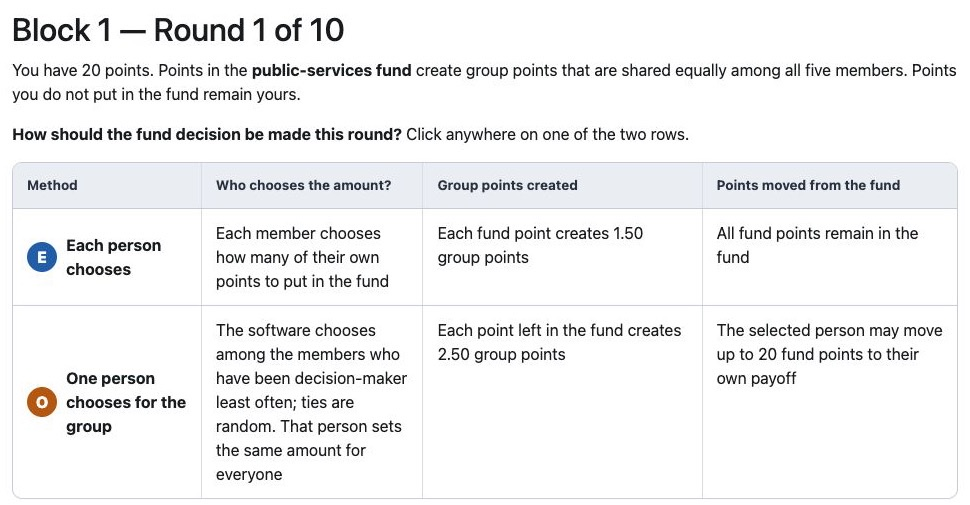
\includegraphics[width=0.98\linewidth]{../../figures/interface_institution_choice.jpg}
\caption{Method ballot. Participants compare the approval rule, fund rate, and consequence of rejection, then select a row. The leader is chosen only after this ballot.}
\end{figure}

\begin{figure}[H]
\centering
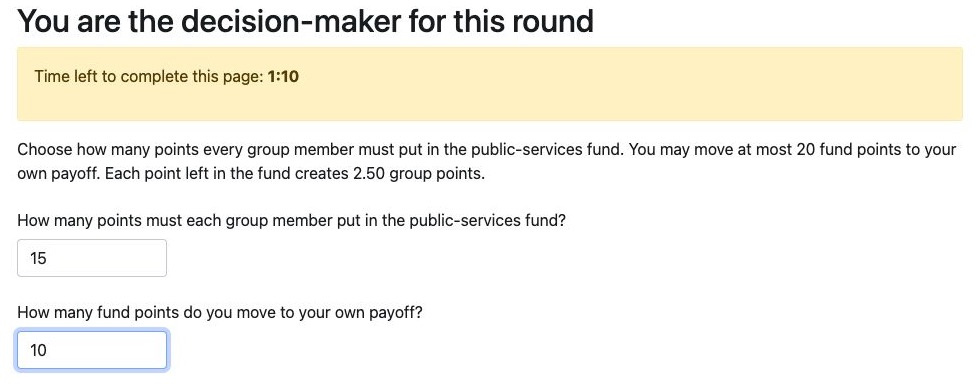
\includegraphics[width=0.98\linewidth]{../../figures/interface_leader_allocation.jpg}
\caption{Leader proposal. The selected participant proposes the common fund allocation and any transfer to their own payoff. The screen states whether approval is required and shows the applicable fund rate.}
\end{figure}

\clearpage
\begin{figure}[H]
\centering
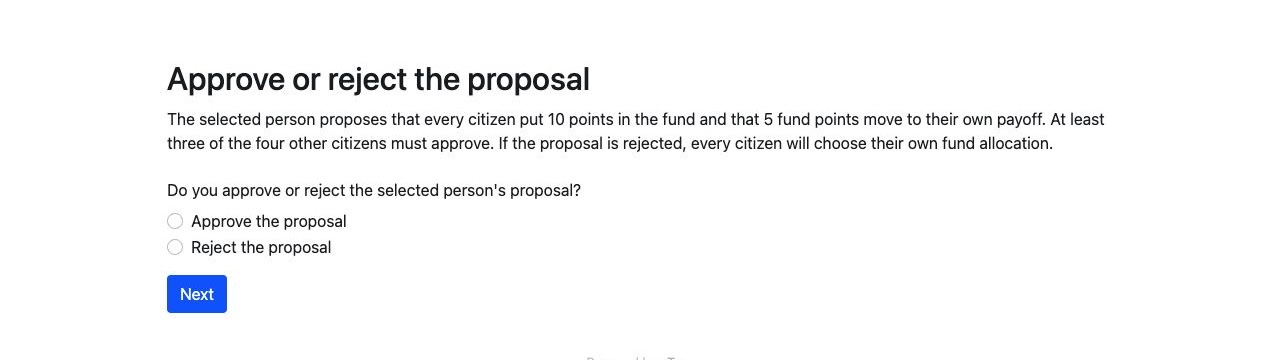
\includegraphics[width=0.98\linewidth]{../../figures/interface_individual_allocation.jpg}
\caption{Approval decision. When group approval is required, each of the four nonleaders sees the complete proposal and chooses approve or reject. At least three approvals are required.}
\end{figure}

\begin{figure}[H]
\centering
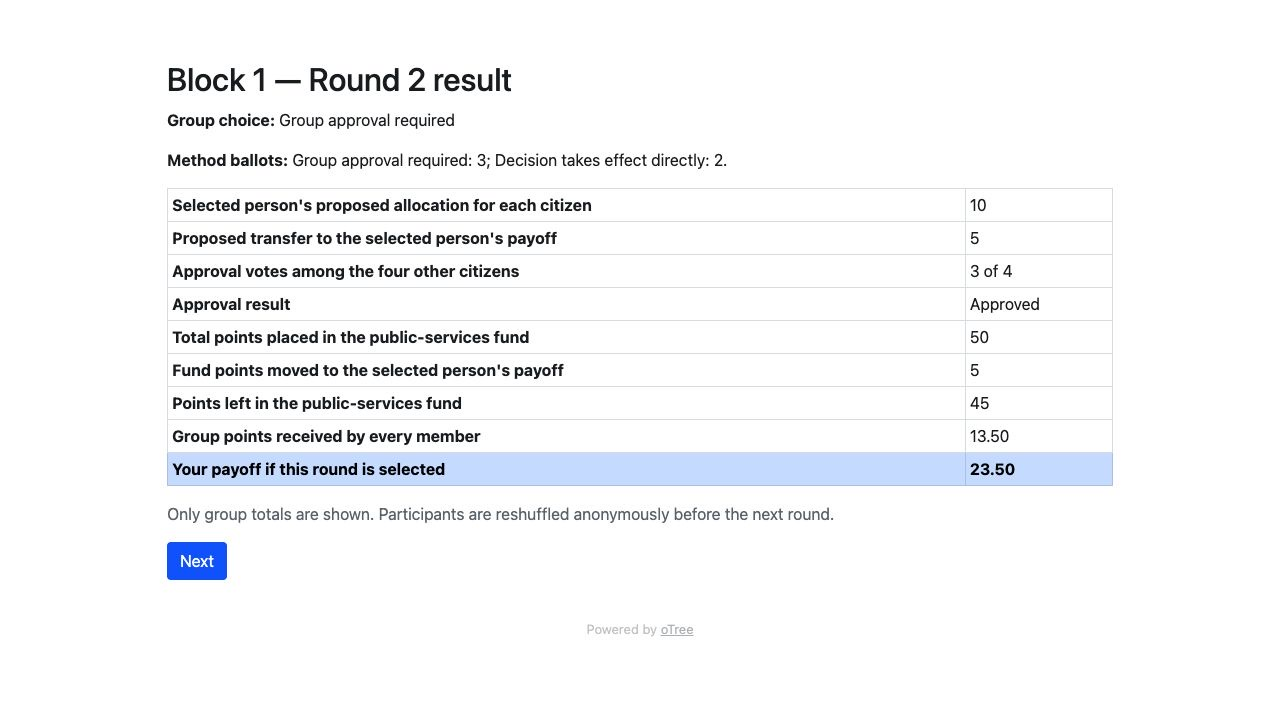
\includegraphics[width=0.95\linewidth]{../../figures/interface_round_result.jpg}
\caption{Round feedback. Participants see the chosen method, aggregate ballots, proposal and approval outcome, fund totals, group return, and their own potential payoff. No participant identity is displayed.}
\end{figure}

\end{document}
